% Problem 3a sketch: shell mass balance on species A in the stagnant liquid film
% Compile with pdflatex; this file makes a standalone figure.
\documentclass[border=6pt]{standalone}
\usepackage{amsmath}
\usepackage{tikz}
\usetikzlibrary{arrows.meta, patterns}
\begin{document}
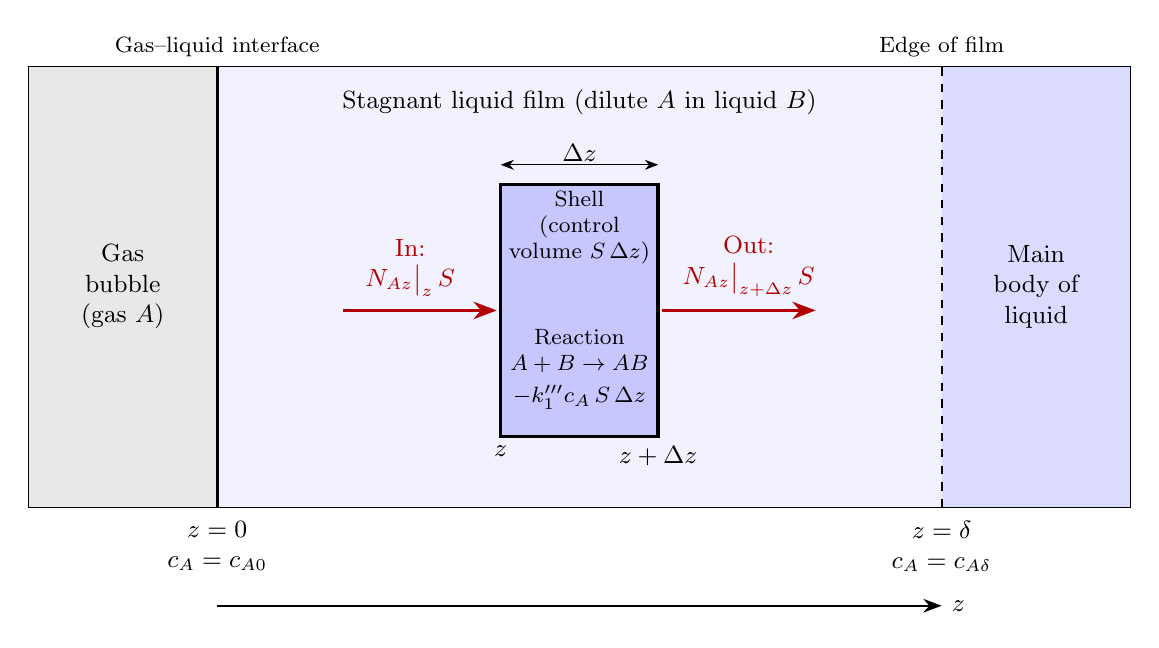
\begin{tikzpicture}[>=Stealth, font=\small]

    % Regions: gas bubble | stagnant liquid film | main body of liquid
    \fill[gray!18]  (0, 0) rectangle (2.4, 5.6);
    \fill[blue!5]   (2.4, 0) rectangle (11.6, 5.6);
    \fill[blue!14]  (11.6, 0) rectangle (14.0, 5.6);
    \draw[very thick] (2.4, 0) -- (2.4, 5.6);
    \draw[thick, dashed] (11.6, 0) -- (11.6, 5.6);
    \draw (0, 0) rectangle (14.0, 5.6);

    \node[align=center] at (1.2, 2.8)  {Gas\\bubble\\(gas $A$)};
    \node[align=center] at (7.0, 5.15) {Stagnant liquid film (dilute $A$ in liquid $B$)};
    \node[align=center] at (12.8, 2.8) {Main\\body of\\liquid};

    % Shell (control volume) between z and z + dz
    \fill[blue!22] (6.0, 0.9) rectangle (8.0, 4.1);
    \draw[very thick] (6.0, 0.9) rectangle (8.0, 4.1);
    \node[align=center, font=\footnotesize] at (7.0, 3.55) {Shell\\(control\\volume $S\,\Delta z$)};
    \node[align=center, font=\footnotesize] at (7.0, 1.75) {Reaction\\$A + B \rightarrow AB$\\[2pt]$-k_1''' c_A\, S\,\Delta z$};

    % Flux in at z and flux out at z + dz (both drawn in +z; N_Az is positive in +z)
    \draw[->, very thick, red!70!black] (4.0, 2.5) -- (5.95, 2.5);
    \node[above, red!70!black, align=center] at (4.85, 2.55) {In:\\$N_{Az}\big|_{z}\, S$};
    \draw[->, very thick, red!70!black] (8.05, 2.5) -- (10.0, 2.5);
    \node[above, red!70!black, align=center] at (9.15, 2.55) {Out:\\$N_{Az}\big|_{z+\Delta z}\, S$};

    % Shell thickness
    \draw[<->] (6.0, 4.35) -- (8.0, 4.35) node[midway, above, fill=blue!5, inner sep=1pt] {$\Delta z$};
    \node[below] at (6.0, 0.9) {$z$};
    \node[below] at (8.0, 0.9) {$z + \Delta z$};

    % Boundary values
    \node[below, align=center] at (2.4, -0.05) {$z = 0$\\$c_A = c_{A0}$};
    \node[below, align=center] at (11.6, -0.05) {$z = \delta$\\$c_A = c_{A\delta}$};
    \node[above, font=\footnotesize] at (2.4, 5.6) {Gas--liquid interface};
    \node[above, font=\footnotesize] at (11.6, 5.6) {Edge of film};

    % z axis
    \draw[->, thick] (2.4, -1.25) -- (11.6, -1.25) node[right] {$z$};

\end{tikzpicture}
\end{document}
